\documentclass[letterpaper]{article} % DO NOT CHANGE THIS
\usepackage[preprint]{aaai2027}  % preprint: shows the authors, no copyright block
\usepackage[hyphens]{url}  % DO NOT CHANGE THIS
\usepackage{graphicx} % DO NOT CHANGE THIS
\urlstyle{rm} % DO NOT CHANGE THIS
\def\UrlFont{\rm}  % DO NOT CHANGE THIS
\usepackage{natbib}  % DO NOT CHANGE THIS AND DO NOT ADD ANY OPTIONS TO IT
\usepackage{caption} % DO NOT CHANGE THIS AND DO NOT ADD ANY OPTIONS TO IT
\frenchspacing  % DO NOT CHANGE THIS

\usepackage{amsmath,amssymb}
\usepackage{booktabs}

\pdfinfo{
/TemplateVersion (2027.2)
}

\setcounter{secnumdepth}{0}

\title{Local and Hosted Models for SOC Alert Triage Under Limited Human Review}
\author{
    Yaniv Zimmer\textsuperscript{\rm 1},
    Yuval Goldberg\textsuperscript{\rm 1},
    Noam Cohen\textsuperscript{\rm 1}
}
\affiliations{
    \textsuperscript{\rm 1}Torq\\
    {firstname.lastname}@torq.io
}

\begin{document}

\maketitle

\begin{abstract}
Modern SOC systems widely use LLMs to automate analysts' alert triage. However, they are far from perfect, and often require a human in the loop to correct their decisions. We investigate whether those corrections can train an in-house model of an organization's triage preferences. Such a model removes the dependence on external frontier models for triage, letting even small organizations, including those constrained by data sovereignty concerns, benefit from automated alert triage. It also avoids per-query API costs and, with fixed weights, returns the same verdict for the same alert, whereas sampled LLM outputs can vary between runs. We compare classifiers trained locally on each organization's labels (fine-tuned encoders, our Tiny Decision, a small decoder classifier built on Qwen3-0.6B, and nearest-neighbor and gradient-boosting models) with systems used without training: hosted classification APIs (OpenAI's Decisions API and TypeSafe's Jev) and prompted LLMs, on 1,492 analyst-labeled production alerts from three tenants and on a 12-organization task derived from the public GUIDE dataset. Each method automates its 80\% most confident alerts and defers the rest to analysts, assumed to review them correctly. Local classifiers made far fewer false escalations while staying competitive on missed malicious alerts: on GUIDE, Tiny Decision missed as many malicious cases as the strongest hosted configuration (12 each) with a third of its false escalations (30 versus 90). On production alerts, the best hosted API missed fewer malicious alerts but escalated several times more benign ones. These results support small local models as a first-stage alternative for alert triage in incident-response workflows.
\end{abstract}

\begin{links}
    \link{Code and data}{https://github.com/YanivZimmer/SocTriage}
\end{links}

\section{Introduction}

Most alerts that SOC analysts see need no action \citep{alahmadi2022falsepositives}, so triage is an obvious target for automation. Although SOC triage is a classification problem, several properties distinguish it from ordinary classification and motivate dedicated research. In cyber defense, and specifically in SOC triage, errors are asymmetric: a malicious alert incorrectly closed without review leaves a possible intrusion unexamined, and can pose an imminent threat, while a benign alert escalated as malicious costs analyst and incident response time, where talent is short and their time is very limited. As a result, pressure to automate triage is high, and automated verdicts may go unreviewed. To that end, we conducted a comprehensive evaluation, using both public and proprietary data, aiming to address these failure points and give practitioners and researchers a better understanding of the field. 

A SOC triage system has two broad options. One option, which may involve less deployment friction, is to send alerts to an external model, either a frontier LM or a classification API such as Jev or the Decisions API, that returns a verdict with a confidence score. Prompted LLMs, however, can return different verdicts for identical inputs \citep{atil2024nondeterminism}, and their stated confidence is coarse and poorly calibrated \citep{xiong2024uncertainty}, a weak basis for deciding which alerts an analyst should review. Alternatively, an organization can train a text model on its own data, either from scratch or by adapting an open-weight model. Prominent options include fine-tuned encoders such as ModernBERT \citep{warner2024modernbert} and tiny decision models (such as the one we present) based on open-weight decoder models, using a classification head at inference instead of an autoregressive head. 

While the second option requires more deployment effort, we show it can be very beneficial; it also avoids per-query API costs and keeps alerts inside the organization.

Additionally, we evaluated a variant of the first option in which external models receive few-shot exemplars: the most similar past alerts, retrieved with their verdicts. We show that this strategy improves their performance and can offer a middle ground for practitioners concerned primarily with performance and minimal deployment effort.

These approaches reuse analyst judgment in different ways. Historical verdicts record how a team interprets alerts in its own environment, including which recurring activities are expected and which warrant investigation. Local training incorporates that judgment into a tenant-specific model; retrieval supplies selected past decisions as context for each hosted query. The practical question is how effectively these uses of analyst history support consistent triage while reserving limited review capacity for uncertain cases. Our comparison evaluates their error trade-offs under the same review budget.

Our contributions are:

\begin{itemize}
    \item A comparison of six local classifiers, two hosted classification APIs with zero to 20 exemplars and prompted LLMs on private production alerts from three tenants and on a 12-organization task derived from GUIDE \citep{guide2024}, whose construction code and per-prompt model outputs we release, with organization-level summaries and sensitivity analyses for label weighting, duplication, an outcome-bearing field and later data. The local classifiers closed more non-malicious alerts without review on both datasets, with similar observed miss counts on GUIDE and with more unreviewed misses on production.
    \item An evaluation protocol, applied consistently to every method in this study, for comparing triage models and variants at a fixed review budget, which differs from a fixed numerical confidence threshold: the primary comparison automates each method's most-confident 80\% within every evaluated batch, while thresholds selected on validation data are fixed in advance and may reach a different test coverage. We report workflow precision and recall, unreviewed misses and false escalations as counts with their denominators, and noise reduction (the share of non-malicious alerts closed without review) under an explicit ideal-review assumption.
    \item A short ablation of a recall-oriented hinge loss, which helped when training batches were not rebalanced.
\end{itemize}

\paragraph{Closest prior work.} AACT \citep{turcotte2025aact} trains a supervised model on analysts' past triage actions and automates part of the alert stream, which is the local option we evaluate; CORTEX \citep{wei2025cortex} automates triage with LLM agents, and DeepCASE \citep{vanede2022deepcase} routes uncertain event sequences to operators. LLMs are now proposed for many SOC tasks \citep{habibzadeh2026survey,singh2026llms}. AACT and CORTEX also report comparative evaluations. We compare locally trained classifiers and hosted model configurations on common inputs under a shared deferral budget, and examine whether validation-selected thresholds preserve that budget on later data. We use the reject option of selective classification, which established the general deferral framework \citep{chow1970reject,geifman2017selective}; learning to defer \citep{mozannar2020defer} trains the deferral policy, which we do not. 

\section{Task and Evaluation Protocol}

\paragraph{Task.} Each alert has an analyst verdict: false positive (the detection fired incorrectly), true positive benign (authorized activity) or true positive malicious. The boundary between the first two is a matter of the tenant's security policy, so we make the task policy-agnostic: binary classification of malicious (true positive malicious) versus non-malicious (false positive or true positive benign). A method's \emph{verdict} is malicious or non-malicious; its \emph{confidence} is a score used to rank alerts and show the analyst which ones they should review carefully.

\paragraph{Automation and deferral.} A \emph{gate} decides, per alert, whether the model's verdict is applied automatically or the alert is deferred to an analyst. We rank alerts by confidence: the largest class probability for local classifiers and open LLMs, the API's own verdict confidence for classification APIs, and the stated confidence for prompted hosted LLMs. A gate automates the highest ranked alerts. We assume that deferred alerts receive correct verdicts. This is in part an idealization: it measures what automation loses, not what analysts achieve.

\paragraph{Workflow metrics.} Over all evaluated alerts we form one confusion matrix: TP = automated true positives + deferred malicious alerts; FN = malicious alerts automated as non-malicious; FP = non-malicious alerts automated as malicious; TN = automated true negatives + deferred non-malicious alerts. FN are \emph{unreviewed misses} and FP are \emph{false escalations}. We report both counts with their denominators, \emph{workflow precision} TP/(TP+FP), \emph{workflow recall} TP/(TP+FN), and the \emph{automation rate}, the share of alerts decided without review. We also report noise reduction, the share of non-malicious alerts closed automatically (automated with a non-malicious verdict). Because deferred alerts count as correct, workflow recall rises mechanically with deferral. Automation is not the same as workload reduction: escalated alerts, true or false, still reach analysts or incident responders, and review time differs between alerts.

\paragraph{Two ways to set the gate.} The primary comparison is \emph{retrospective matched coverage}: for each organization or tenant-fold, the gate automates the $\lceil 0.8n\rceil$ highest-ranked test alerts (ties broken by alert identifier), so every method defers the same number of alerts. This is a review-budget target, not a fixed confidence threshold: it compares rankings at an equal review budget. Such a batch-quantile policy can be deployed, but this comparison does not establish that a threshold selected on earlier data will preserve this review budget on future alerts. Second, validation-selected numerical thresholds are fixed on each validation split and transferred: a deferral threshold at the confidence that automates 80\% of validation alerts, and full-automation thresholds on $p(\text{malicious})$ at a target validation false-positive rate (FPR). Their test automation and error rates are what they achieve, not matched. The threshold targets and statistical tests were fixed in a written reanalysis plan before these test outcomes were computed, but after earlier results on the same data were known, so this analysis is not confirmatory.

\paragraph{Ranking is not calibration.} The gate uses only the order of confidences. We make no claim that any method's confidence is a calibrated probability \citep{guo2017calibration}, and verbalized LLM confidences are known to be poorly calibrated \citep{xiong2024uncertainty}.

\paragraph{Uncertainty.} On GUIDE the organization is the unit of replication: we report per-organization wins and losses with exact Wilcoxon signed-rank tests and an organization-cluster bootstrap (2,000 replicates). Local models were trained with one seed on GUIDE, so these intervals do not include training variation. Production has three tenants, so production results are descriptive; where available we report variation over training seeds and the released alert-level bootstrap intervals, which resample alerts within tenant and fold. Neither repeated seeds nor overlapping folds are independent deployments.

\section{Data and Compared Systems}

\paragraph{Production alerts.} We use 1,492 alerts from three tenants, A, B and C (412, 707 and 373 alerts; 17, 39 and 17 malicious), collected between September 2025 and September 2026. Every label is an analyst verdict given after a production LLM (Gemini 2.5 Pro with the production prompt) had triaged the alert: 528 labels correct that LLM's verdict, only six of them to malicious, and 943 of the 964 uncorrected labels equal its verdict. The labels therefore measure agreement with analysts who saw an LLM verdict, not independently verified attacks. Analysts chose which alerts to review, which may not be random with respect to the verdict. Each tenant is split into three folds stratified by label; 15\% of each training fold is held out for validation. Folds are random rather than time-ordered, and alerts repeat: 33.5\% of tenant A's test alerts have a near-identical alert in training. We test the effect of duplicates and of later data below and discuss it under Limitations. Alerts are serialized from 21 fields (e.g., alert name, observables with threat-intelligence enrichment, process chain, command line and the vendor's \emph{Response} field); the label, analyst comment and LLM verdict are never included. On tenant A one Response value alone identifies 7 of the 17 malicious alerts with no false positives, so this field can carry outcome information. Tenant A's analysts later reviewed 433 further alerts (11 malicious), which we use as later data.

\paragraph{GUIDE-derived task.} GUIDE \citep{guide2024} contains Microsoft security incidents graded TruePositive, BenignPositive or FalsePositive. Our task transforms it in four ways that matter for interpretation. (1) The released train and test files are pooled and re-split, so our splits are not GUIDE's. (2) Each incident's evidence rows are aggregated into a record with only categorical content, rendered into a description of the form \texttt{evidence\_count=N | categories=\ldots{} | mitre\_techniques=\ldots{} | entity\_types=\ldots{} | evidence\_roles=\ldots}; there are no command lines, file names or free text, and incidents with conflicting grades are dropped. (3) Incidents with byte-identical text collapse into one \emph{prompt}, the unit of prediction: in the 12 organizations, 71,576 incidents become 7,160 prompts, a prompt takes the majority grade of its incidents (ties broken toward malicious), 414 prompts (5.8\%) have mixed grades, and 3.2\% of incidents disagree with their prompt's label. (4) Twelve organizations were chosen in a pre-registered hash order among those with at least 300 prompts and 10 malicious ones, and each is split 70/15/15 by prompt. The test sets hold 1,079 prompts (456 malicious, 623 non-malicious) from 9,722 incidents; repetition is uneven, as the 11 largest prompts hold 52\% of the test incidents. All GUIDE counts and automation rates in this paper are per prompt unless stated otherwise: automating 80\% of test prompts is not automating 80\% of incidents. Labels are Microsoft's grades, independent of our production LLM.

\paragraph{Compared systems.} Table~\ref{tab:methods} lists the methods. Local classifiers are trained per tenant or organization on the training split (one seed on GUIDE). Hosted APIs and LLMs receive the same serialized alert and, optionally, exemplars: the most similar training alerts with their labels, retrieved without looking at the query's label. Some production-only local variants (focal-Tversky \citep{abraham2019focaltversky}, SetFit \citep{tunstall2022setfit}, RiskFit hyperparameter variants) are reported in the release, not here. All results come from existing predictions and model outputs; no model was retrained or queried again for this analysis.

\begin{table}[t]
\centering
\small
\begin{tabular}{@{}p{0.25\columnwidth}p{0.66\columnwidth}@{}}
\toprule
Method & Description (gate confidence) \\
\midrule
\multicolumn{2}{@{}l}{\emph{Locally trained classifiers}} \\
CE & SecureBERT 2.0 \citep{aghaei2025securebert2} + LoRA \citep{hu2022lora}, cross-entropy and supervised contrastive loss \citep{khosla2020supcon}, class-balanced batches (max.\ prob.) \\
RiskFit & CE plus a hinge on soft malicious recall (Eq.~\ref{eq:riskfit}) \\
Tiny Decision & Qwen3-0.6B \citep{qwen3} + LoRA with a classification head (max.\ prob.) \\
MaxSim & FastFit similarity classifier \citep{yehudai2024fastfit} \\
$k$NN & $k{=}5$ over frozen SecureBERT embeddings \\
LightGBM & gradient boosting \citep{ke2017lightgbm} on structured fields \\
\midrule
\multicolumn{2}{@{}l}{\emph{Hosted classification APIs (no training)}} \\
Decisions & OpenAI Decisions API \citep{openai2026decisions}, \texttt{gpt-6-luna}; 0 or 1 exemplar; GUIDE also 5 and 20 (API confidence) \\
Jev & TypeSafe Jev \citep{typesafe2026jev}, \texttt{jev-1.14.0}; GUIDE only; 0, 1, 5, 20 exemplars \\
\midrule
\multicolumn{2}{@{}l}{\emph{Prompted LLMs}} \\
Gemini & Gemini 2.5 Pro \citep{gemini25}; production only; 0 or 1 exemplar (stated conf.) \\
Opus & Claude Opus 5.5 \citep{anthropic2026opus55}; GUIDE test set only; 0 or 1 exemplar (stated conf.) \\
CyberSecQwen & 4B open security LLM \citep{athena2026cybersecqwen}, run locally, zero-shot (label likelihood) \\
\bottomrule
\end{tabular}
\caption{Compared systems. Exemplars are retrieved, label-blind, from the training split and shown with their labels.}
\label{tab:methods}
\end{table}

\section{Results}

\begin{table}[t]
\centering
\small
\begin{tabular}{@{}lrrrr@{}}
\toprule
Method & Miss & FE & W.~prec. & W.~rec. \\
\midrule
\multicolumn{5}{@{}l}{\emph{GUIDE: 1,079 prompts; 868 automated (80.4\%)}} \\
RiskFit & 11 & 46 & .906 & .976 \\
CE & 15 & 35 & .926 & .967 \\
Tiny Decision & 12 & 30 & .937 & .974 \\
$k$NN & 21\textsuperscript{a} & 28 & .940 & .954 \\
LightGBM & 31 & 39 & .916 & .932 \\
MaxSim & 38 & 17 & .961 & .917 \\
Decisions, 0-shot & 0 & 497 & .478 & 1.000 \\
Decisions + 1 ex. & 8 & 420 & .516 & .982 \\
Decisions + 5 ex. & 24 & 109 & .799 & .947 \\
Decisions + 20 ex. & 12 & 90 & .831 & .974 \\
Jev + 20 ex. & 29 & 213 & .667 & .936 \\
Opus + 1 ex. & 16\textsuperscript{a} & 241 & .646 & .965 \\
CyberSecQwen & 0 & 502 & .476 & 1.000 \\
\midrule
\multicolumn{5}{@{}l}{\emph{Production: 1,492 alerts; 1,197 automated (80.2\%)}} \\
RiskFit & 9 & 28 & .696 & .877 \\
CE & 9 & 8 & .889 & .877 \\
Tiny Decision & 10 & 5 & .926 & .863 \\
$k$NN & 16 & 2 & .966 & .781 \\
LightGBM & 13 & 6 & .909 & .822 \\
MaxSim & 7 & 4 & .943 & .904 \\
Decisions, 0-shot & 1 & 945 & .071 & .986 \\
Decisions + 1 ex. & 0 & 154 & .322 & 1.000 \\
Gemini + 1 ex. & 11 & 41 & .602 & .849 \\
\bottomrule
\end{tabular}
\caption{Fixed review budget (retrospective matched coverage): every method automates its 80\% most confident alerts per organization or tenant-fold. Miss: unreviewed malicious misses, a count (GUIDE: of 456 malicious prompts; production: of 73 malicious alerts); FE: false escalations, a count (GUIDE: of 623 non-malicious prompts; production: of 1,419 non-malicious alerts); workflow precision and recall assume deferred alerts are resolved correctly. One training seed (seed 42 on production). \textsuperscript{a}Depends on tie order at the cutoff: $k$NN 19--21, Opus 10--21 misses (241: 236--251 FE).}
\label{tab:main}
\end{table}

\subsection{Comparison at a Fixed Review Budget}

Table~\ref{tab:main} gives the primary comparison. Local classifiers closed more non-malicious alerts without review on both datasets; what that cost in missed malicious alerts differs between them.

On GUIDE, the best local classifiers (RiskFit, Tiny Decision, CE) left 11 to 15 of 456 malicious prompts unreviewed and misclassified, with 30 to 46 false escalations. The hosted configurations with zero or one exemplar and CyberSecQwen missed 0 to 16 malicious prompts (Jev with one exemplar: 27) but escalated 241 to 502 of the 623 non-malicious ones, producing many false escalations (workflow precision .48--.65). More exemplars changed this: with 20, the Decisions API missed 12 prompts with 90 false escalations, the strongest hosted result. Against it, the local classifiers' miss counts were not consistently lower (RiskFit fewer in 3 organizations, more in 3, tied in 6; Wilcoxon $p{=}0.97$), but their false escalations were lower in most organizations (CE and Tiny Decision: 10 of 12, $p{=}0.005$; RiskFit: 7 lower, 2 higher, 3 tied, $p{=}0.066$; unadjusted). Workflow recall was .976 (95\% interval .948--.991) with 46 false escalations (21--71) for RiskFit and .974 (.926--.993) with 90 (47--137) for Decisions + 20 exemplars: the variation across organizations is large relative to the difference. Jev with 20 exemplars missed more (29) and escalated more (213) than the local classifiers.

On production alerts the pattern is a trade-off rather than an ordering. The Decisions API with one exemplar missed none of the 73 malicious alerts but made 154 false escalations; the local classifiers missed 7 to 16 with 2 to 28 false escalations, so their workflow precision was higher and their workflow recall lower. Gemini with one exemplar missed 11 with 41 false escalations, and its stated confidence took at most six distinct values per fold, which makes its gate sensitive to ties. Training seeds matter for the local results: over seven seeds, RiskFit's 80\% gate missed 9.3 $\pm$ 2.0 alerts (range 5--11) with 16.0 $\pm$ 6.2 false escalations (9--28), and CE's (rerun on RiskFit's GPU) 9.3 $\pm$ 2.6 with 11.3 $\pm$ 3.4; the seed in Table~\ref{tab:main} is RiskFit's worst for false escalations.

\paragraph{Noise reduction.} At this budget the local classifiers closed more non-malicious alerts without review than the strongest hosted configuration on both datasets: 69--80\% of non-malicious GUIDE prompts against 63\% for Decisions + 20 exemplars, and 78--82\% of non-malicious production alerts against 69\% for the Decisions API with one exemplar. On GUIDE the best of them (RiskFit, CE, Tiny Decision) did so at about the same workflow recall (.967--.976 against .974); on production the extra noise reduction came with 7 to 16 unreviewed misses of 73, against none.

\paragraph{Confidence ranking (production).} The gate helps only if a method's confidence separates the alerts it gets right from those it gets wrong. For RiskFit it does: lowering coverage from 100\% to 80\% raised the accuracy of the automated alerts from 91.0\% to 96.1\% on tenant A, from 75.1\% to 79.7\% on tenant B and from 95.4\% to 99.7\% on tenant C. Unlike workflow recall, this does not rely on the assumption that analysts resolve deferred alerts correctly. Gemini with one exemplar did not show this on tenant B (51.3\% at full coverage, 50.5\% at 80\%), consistent with its coarse stated confidence. Ranking is distinct from calibration: a score can order alerts well without being an accurate probability.

\paragraph{Weighted error cost.} If one miss is weighted as $c$ false escalations, the weighted error cost is $c\cdot\text{misses}+\text{false escalations}$; $c$ is a ratio of error weights, not money \citep{elkan2001costsensitive}. On production alerts the Decisions API with one exemplar has a lower weighted cost than RiskFit for $c$ above about 14, than CE above about 16 and than MaxSim above about 21 (alert-bootstrap interval for MaxSim 11--71). On GUIDE, RiskFit and Tiny Decision have no more misses and fewer false escalations than Decisions + 20 exemplars, so they have a lower weighted cost at every $c$; CE has a lower one up to $c\approx18$. Our analysts' prior rule of thumb was $c\le10$, but $c$ differs between teams and alert types.

\begin{figure*}[t]
\centering
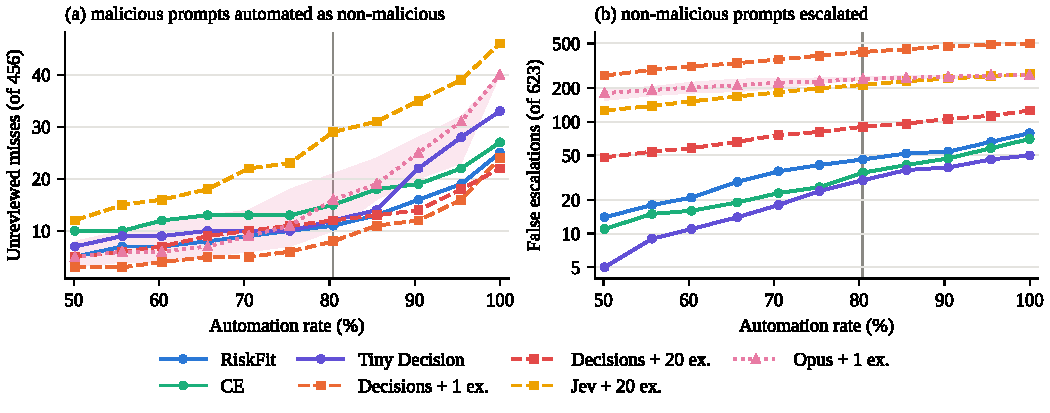
\includegraphics[width=\textwidth]{figures/guide_automation_sweep.pdf}
\caption{GUIDE, retrospective matched coverage at automation rates from 50\% to 100\%: (a) unreviewed malicious misses (of 456) and (b) false escalations (of 623, log scale), pooled over 12 organizations. Solid: local classifiers; dashed: classification APIs; dotted: Opus, with the range over tie orders shaded. The vertical line marks the 80\% budget of Table~\ref{tab:main}.}
\label{fig:sweep}
\end{figure*}

\subsection{Performance Across Automation Rates}

Figure~\ref{fig:sweep} repeats the GUIDE comparison from 50\% to 100\% automation. The orderings of Table~\ref{tab:main} do not all hold at every rate (some curves tie or cross), but false escalations stay broadly separated: at every rate, the hosted configurations with at most one exemplar and Jev with 20 made at least 120 false escalations, Decisions with 20 exemplars made 48 to 126, and the three local classifiers made 5 to 79. Misses rise steeply above 85\% automation for every method; above 80\%, the Decisions API with one or 20 exemplars missed slightly fewer malicious prompts than the local classifiers (at 90\%: 12 and 14 against 16 to 22). With no deferral (100\%), RiskFit missed 25 with 79 false escalations, CE 27 with 70, Tiny Decision 33 with 50, Decisions + 20 exemplars 22 with 126 and Decisions + 1 exemplar 24 with 500. On production alerts with no deferral, the Decisions API with one exemplar missed 2 of 73 with 213 false escalations, RiskFit 17 with 64 and CE 22 with 36; deferring 20\% removed about half of the local models' misses and about a quarter of the hosted API's false escalations. Production per-alert scores are not released, so we cannot sweep production automation rates beyond these two points.

\subsection{Validation-Selected Thresholds and Later Data}

\begin{table}[t]
\centering
\small
\begin{tabular}{@{}lrrrrr@{}}
\toprule
Method & Auto. & Miss & FE & W.~prec. & W.~rec. \\
\midrule
\multicolumn{6}{@{}l}{\emph{GUIDE (of 456 / 623)}} \\
RiskFit & 79.3\% & 12 & 47 & .904 & .974 \\
CE & 80.2\% & 15 & 33 & .930 & .967 \\
Tiny Decision & 80.4\% & 13 & 33 & .931 & .971 \\
Decisions + 1 ex. & 81.0\% & 10 & 416 & .517 & .978 \\
Decisions + 20 ex. & 79.6\% & 11 & 87 & .836 & .976 \\
Jev + 20 ex. & 83.5\% & 31 & 223 & .656 & .932 \\
\midrule
\multicolumn{6}{@{}l}{\emph{Production (of 73 / 1,419)}} \\
RiskFit & 74.5\% & 6 & 26 & .720 & .918 \\
CE & 77.9\% & 9 & 8 & .889 & .877 \\
MaxSim & 78.7\% & 7 & 4 & .943 & .904 \\
LightGBM & 77.5\% & 14 & 4 & .937 & .808 \\
Decisions + 1 ex. & 81.7\% & 0 & 155 & .320 & 1.000 \\
\midrule
\multicolumn{6}{@{}l}{\emph{Tenant A, later alerts (of 11 / 422)}} \\
RiskFit & 20.1\% & 2 & 0 & 1.000 & .818 \\
CE & 15.2\% & 1 & 2 & .833 & .909 \\
LightGBM & 71.8\% & 2 & 0 & 1.000 & .818 \\
Decisions + 1 ex. & 39.0\% & 0 & 20 & .355 & 1.000 \\
Decisions, 0-shot & 92.8\% & 0 & 268 & .039 & 1.000 \\
\bottomrule
\end{tabular}
\caption{Deferral threshold set on validation (the confidence that automates 80\% of validation alerts) and applied unchanged; Auto.\ is the automation rate actually achieved on the test or later alerts, so rows are not workload-matched. Opus has no validation outputs and is omitted. Later alerts: models trained, and exemplars drawn, from tenant A's earlier alerts.}
\label{tab:transfer}
\end{table}

Table~\ref{tab:transfer} applies deferral thresholds chosen on validation data. Pooled automation remained near the target within the benchmarks (78--84\% on GUIDE, 74.5--84.5\% on production), although GUIDE organization-level rates ranged from 60\% to 98\%, and the errors resemble Table~\ref{tab:main}. On tenant A's later alerts they did not: the same rule automated 15\% (CE), 20\% (RiskFit), 39\% (Decisions + 1 exemplar), 72\% (LightGBM) and 93\% (zero-shot Decisions) of alerts. A threshold that defers few alerts on earlier data can defer most of them later, or the reverse, so a deployment would need to monitor and re-set it. For reference, when 80\% of these later alerts were automated retrospectively, RiskFit missed 2 of 11 with 1 false escalation, LightGBM 2 with 0, CE 2 with 28 and the Decisions API with one exemplar 1 with 56; with 11 malicious alerts these differences are only indicative. The API's false-escalation rate at its default verdict rose from 0.045 on the benchmark to 0.18 on the later alerts, while 66\% of the later alerts had no retrieved exemplar above the similarity threshold (38\% before). A later tenant C export omitted severity for many alerts and used a different non-malicious labeling convention, so we excluded it from the clean temporal comparison. It nevertheless exposed sensitivity to export changes: RiskFit falsely escalated 295 of 1,034 non-malicious alerts at its default verdict.

Without deferral, thresholds on $p(\text{malicious})$ set on validation data at RiskFit's validation FPR gave no detected difference in per-organization GUIDE recall between RiskFit or CE and Decisions + 20 exemplars (Holm-adjusted \citep{holm1979}, $p{\ge}0.39$), which does not establish equivalent ranking; a fixed 5\% validation FPR lowered recall for every method.

\subsection{Sensitivity to Weighting, Duplication and Leakage}

\paragraph{Incident weighting (GUIDE).} Our GUIDE results count prompts, but an analyst's queue holds incidents, and one prompt stands for anywhere from one to 1,317 of them. To test whether the conclusions depend on this unit, we keep each method's decisions from the 80\% prompt-level gate and count incidents instead: every incident inherits its prompt's automation decision and verdict. This is a sensitivity analysis, as specified in the reanalysis plan; the primary comparison keeps prompts as the unit. Every method still automates 868 of 1,079 test prompts, but each picks its own 868, the prompts it is most confident about, so the share of incidents automated differs (83.6\% for RiskFit, 72.7\% for CE, 68.0\% for Decisions + 20 exemplars) and incident-review workloads are not matched. Counted this way, RiskFit missed 26 of 4,259 malicious test incidents and CE 30, while Decisions + 20 exemplars missed 535, of which 508 come from a single prompt; in exchange it falsely escalated fewer non-malicious incidents (188 of 5,463, against 581 for RiskFit and 363 for CE). Because 11 prompts hold 52\% of the test incidents, incident-weighted results mostly reflect how each method handles those few prompts, and one decision can dominate the outcome.

\paragraph{Duplication and leakage (production).} Production alerts repeat heavily and folds are random, so a test alert can have a near-copy in training, and one alert field (Response) can reveal the outcome. Either could inflate the results. We ran two test-time checks, without retraining. First, we kept only the 280 test alerts with no training neighbor above cosine similarity 0.95 (37 malicious) and applied the 80\% gate thresholds from the full test set: RiskFit made 4 misses with 7 false escalations, CE 3 with 1, Tiny Decision 5 with 1 and the Decisions API with one exemplar 0 with 66, the same trade-off as in Table~\ref{tab:main}. Second, removing the Response field from the test alerts changed misses at the gate from 9 to 8 for RiskFit, 9 to 10 for CE, 16 to 18 for $k$NN and 0 to 2 for the Decisions API. Neither check changes the picture, but both are limited: the local models were trained with the Response field and on duplicated, randomly split data, and test-time recalculation cannot remove what they learned from it.

\section{Secondary Ablation: A Recall-Oriented Loss}

RiskFit adds a hinge on soft malicious recall to the CE objective. With $p_i$ the predicted probability that alert $i$ is malicious, $\mathcal{M}$ the malicious alerts in a training window and $R_{\text{soft}}=\frac{1}{|\mathcal{M}|}\sum_{i\in\mathcal{M}}p_i$,
\begin{equation}
\mathcal{L} = \mathcal{L}_{\text{CE}} + \gamma\,\mathcal{L}_{\text{SupCon}} + \lambda \max(0, \rho - R_{\text{soft}}),
\label{eq:riskfit}
\end{equation}
with $\rho{=}0.9$, $\lambda{=}2$, $\gamma{=}0.5$, fixed by convention. A pre-registered production experiment crossed sampling (class-balanced micro-batches, as in our recipe, or the data's natural class ratio) with the loss over three seeds (Table~\ref{tab:hinge}); we report it descriptively, because overlapping tenant-folds and repeated seeds are not independent deployments. Under natural sampling, the hinge increased malicious alerts detected from 11.7 $\pm$ 0.6 to 46.0 $\pm$ 4.0 of 73 (seeds: 46, 50, 42; stronger hinges 45.3 and 47.0), with approximately 28.7 additional false escalations. Under balanced sampling, CE detected 47.3 $\pm$ 2.5 and the hinge model 49.3 $\pm$ 3.5; CE alone already drove training soft recall from 0.36 to 0.99, and the hinge was rarely active by the last epoch. In this experiment, the hinge mainly compensated for class imbalance. The recall target $\rho$ did not set the operating point: training with $\rho$ from 0.7 to 0.95 gave test recall 0.72--0.74. Over seven seeds with balanced sampling, RiskFit caught 0.6 more malicious alerts than CE on average and made 9 more false escalations.

\begin{table}[t]
\centering
\small
\begin{tabular}{@{}llcc@{}}
\toprule
Sampling & Loss & Caught (of 73) & FE (of 1,419) \\
\midrule
Balanced & CE & 47.3 $\pm$ 2.5 & 27.0 $\pm$ 6.6 \\
 & + hinge ($\rho$.9/$\lambda$2) & 49.3 $\pm$ 3.5 & 31.3 $\pm$ 4.7 \\
Natural & CE & 11.7 $\pm$ 0.6 & \phantom{0}1.7 $\pm$ 1.5 \\
 & + hinge ($\rho$.9/$\lambda$2) & 46.0 $\pm$ 4.0 & 30.3 $\pm$ 13.1 \\
\bottomrule
\end{tabular}
\caption{Recall hinge by sampling, production alerts at default verdicts: mean $\pm$ standard deviation over three training seeds (each pooled over 9 tenant-folds). With natural sampling the hinge uses soft recall over the 36-alert gradient-accumulation window. Two stronger hinges are in the release.}
\label{tab:hinge}
\end{table}

\section{Discussion and Limitations}

\paragraph{What the evidence supports.} At an equal review budget, local classifiers trained on historical labels successfully closed more non-malicious alerts without review than the strongest hosted configuration tested, on both datasets. On GUIDE they did so at similar miss counts, while hosted configurations with zero or one exemplar escalated most non-malicious prompts; on production alerts the hosted API with one exemplar missed fewer malicious alerts, so there the choice depends on how a SOC weighs the two errors and on whether alerts may leave its infrastructure. When thresholds were set on validation data, tests did not detect a recall difference between the strongest hosted configuration and the local classifiers, which does not establish that they rank alerts equally well. Although the evidence does not show that local models are generally superior, they made far fewer false escalations while staying competitive on misses on GUIDE, and should be considered as a first-stage alternative for SOC triage and potentially other incident-response components.

\paragraph{What it cannot establish.} The production labels are analyst verdicts anchored on a production LLM's verdict, so they measure agreement with that process, not detection of verified attacks, and they may favor models that reproduce the LLM's tendencies. The 80\% comparisons set the cutoff on test data, and the tenant A later-data check, our one clean temporal comparison, shows that thresholds chosen on validation can automate very different shares of new alerts. Folds are random, production data repeat heavily, and one field can reveal the outcome; our test-time checks do not establish performance under a chronological or duplicate-grouped training split \citep{arp2022dos,pendlebury2019tesseract}, which requires retraining. The GUIDE task contains only categorical incident summaries, is dominated by a few highly repeated prompts, and uses Microsoft's grades, so it says little about how hosted models use rich alert text. Four GUIDE organizations have only 3, 4, 13 and 17 non-malicious validation prompts, so a 5\% validation FPR target allows no observed false positive there; they hold 287 of the 456 malicious test prompts, which limits the low-FPR comparison and is not evidence of equivalence. Hosted results rest on one prompt design per model \citep{sclar2024prompt} and, for Opus, one non-deterministic run. Production covers three tenants of one SOC platform and 73 malicious alerts, about six per tenant-fold on tenants A and C.

\paragraph{What deployment would additionally require.} A deployment would need a time-ordered evaluation with its own threshold re-estimation, monitoring of the realized automation rate, audits of automated non-malicious verdicts, a measured analyst accuracy on deferred alerts, and, for local models, a few hundred labeled alerts per tenant and periodic retraining. Retaining new analyst corrections also creates a path to continuous learning through periodic model updates. Newly reviewed alerts can be added to the training history, allowing subsequent updates to reuse the team's accumulated judgment as its environment changes. Earlier analyst decisions can also serve as checks on each update. The present experiments evaluate fixed trained models; repeated feedback and update cycles are a deployment extension. We did not test adaptive attackers, poisoned analyst feedback or prompt injection against hosted models.

\paragraph{Reproducibility.} The Decisions API returned identical outputs on 3,300 repeated production calls; Opus was run once and is not deterministic \citep{atil2024nondeterminism}; the hosted models have no dated snapshots, so a re-query can differ. Local models give repeatable predictions for fixed weights in our runs. Consistency is central to the value of retained analyst feedback: the same input should receive the same verdict until the decision rule is deliberately updated. A locally controlled model lets the SOC retain a fixed version and evaluate each proposed update against earlier analyst decisions before deployment.

\section{Conclusion}

Our evaluation suggests that small, tailored, trained models such as tiny decision models and encoder-based text classifiers can be a real alternative to frontier LMs and proprietary decision models such as Jev and the Decisions API, especially for organizations concerned about data sovereignty and costs.

With a fixed share of alerts sent to analysts, locally trained classifiers closed more non-malicious alerts without review than the strongest hosted configuration tested on each dataset. On the public GUIDE-derived task, the best of them did so at about the same workflow recall; on production alerts, they left more malicious alerts unreviewed, while the strongest alternative, the OpenAI Decisions API (gpt-6-luna) with one exemplar, missed none, but at the cost of many false escalations of benign alerts. Their confidence also picked out their own correct verdicts: RiskFit's automated alerts were more accurate at 80\% coverage than at full coverage on every production tenant, whereas Gemini's stated confidence took at most six values per fold and Opus's ranking depended on tie order.

\section{Ethics and Data Availability}

Alerts were reviewed by analysts in normal SOC operations; no experiment involved human participants. The data owners permitted publication of aggregate results only. Tenants are anonymized, and only Google and OpenAI processed production alerts, with the data owner's approval; TypeSafe and Anthropic saw only public GUIDE data, and the open models ran locally. The public release contains the code and per-prompt GUIDE outputs behind our original analysis and the aggregate production results, and the scripts, inputs and outputs that reproduce every number in this paper. It contains no production alert text, customer identifiers, per-alert predictions or trained adapters.

\bibliography{refs}

\end{document}
